%% Chapter 3: Proposed Methodology

\chapter{PROPOSED METHODOLOGY}

%% ─────────────────────────────────────────────────────────────────────────────
\section{ARCHITECTURAL OVERVIEW}

The proposed system is built on a single architectural decision: \textbf{separate Pareto
front construction (Tier~1) from route selection (Tier~2)}. This separation eliminates
the need to re-run a multi-objective search each time the payload changes. The Pareto
front is computed once for a delivery region and stored. For each new mission, only
Tier~2 runs---reading the payload tag and selecting the appropriate route from the
pre-computed front in near-instantaneous time.

Figure~\ref{fig:sysarch} shows the complete system architecture.

\begin{figure}[tp]
  \centering
  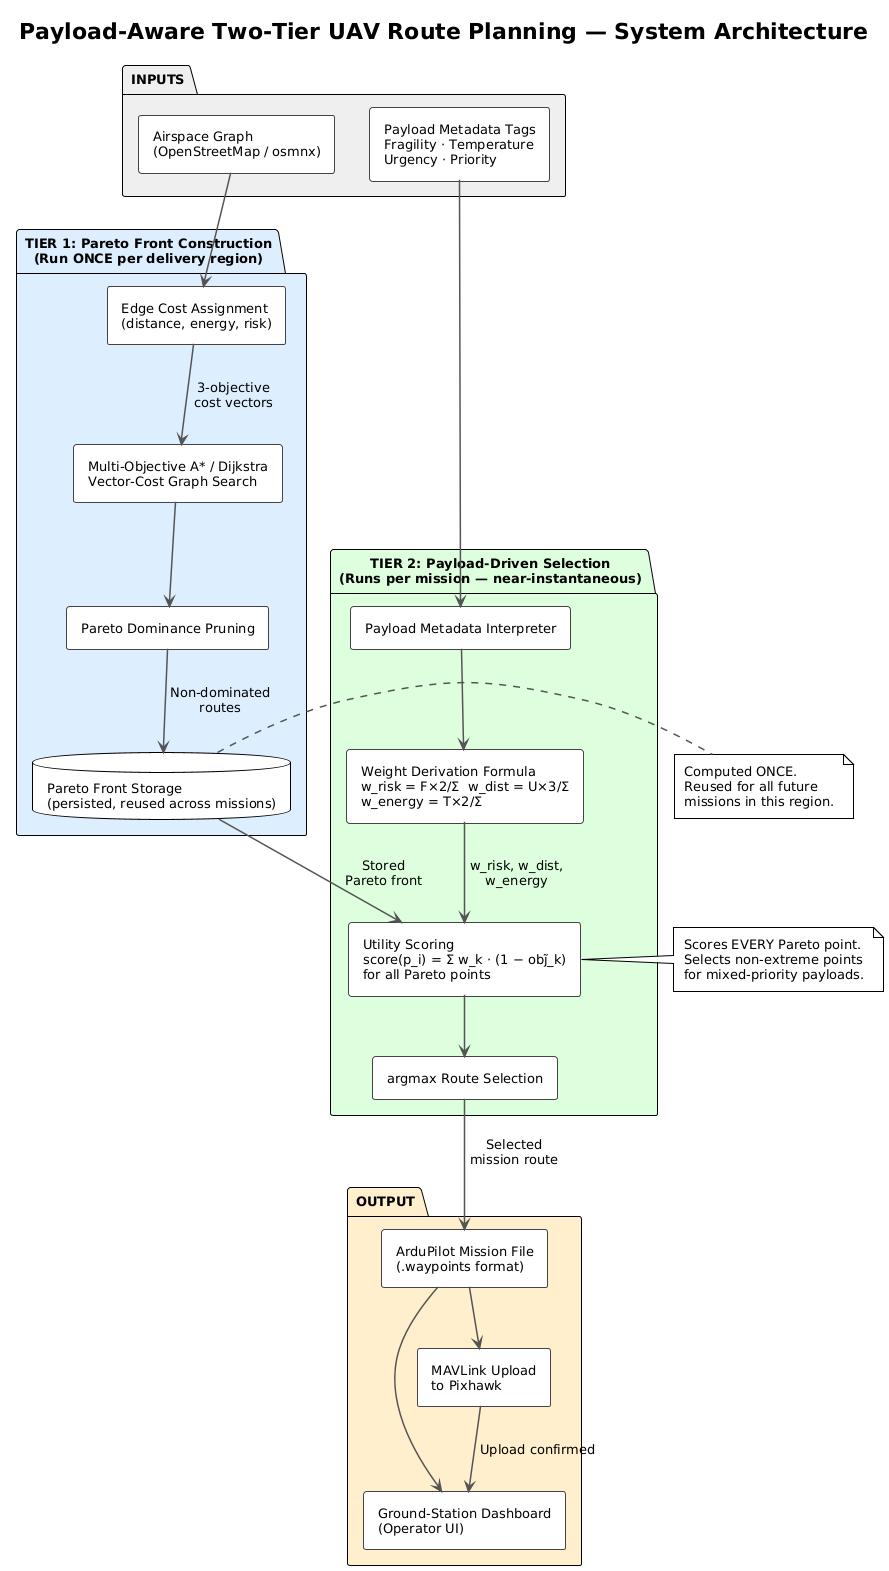
\includegraphics[width=0.70\textwidth]{diagrams/arch.png}
  \caption{Overall System Architecture: Two-Tier Payload-Aware UAV Route Planner.
           Tier~1 pre-computes the Pareto front once; Tier~2 selects the optimal route
           for each new payload tag using the stored front.}
  \label{fig:sysarch}
\end{figure}

%% ─────────────────────────────────────────────────────────────────────────────
\section{TIER 1 --- DETERMINISTIC PARETO FRONT CONSTRUCTION}

\subsection{What Tier 1 Does}

Tier~1 implements a multi-objective A*/Dijkstra graph-search over a delivery airspace
graph. The output is a \textbf{set of Pareto-optimal routes} where no single route
dominates another on all three objectives simultaneously. This front is computed once for
a given delivery region and stored persistently; it does not need to be recomputed
between missions.

\subsection{Airspace Graph Construction}

The airspace graph $G = (V, E)$ is extracted from OpenStreetMap using the
\texttt{osmnx} Python library \cite{osmnx}. Each edge $e \in E$ represents a flight
segment between two waypoints and carries a \textbf{cost vector}:

\begin{equation}
  \mathbf{c}(e) = \bigl[\, d(e),\; \epsilon(e),\; \rho(e) \,\bigr]
\end{equation}

where:
\begin{itemize}
  \item $d(e)$ = geodesic distance of the flight segment (km)
  \item $\epsilon(e)$ = estimated energy consumption (proxy: $d(e) \times$ altitude-change
        factor)
  \item $\rho(e)$ = flight risk score $\in [0, 1]$, derived from obstacle density,
        proximity to no-fly zones, and wind exposure (simulated programmatically for
        reproducible benchmarking)
\end{itemize}

\subsection{Three Optimisation Objectives}

The three routing objectives are:

\begin{enumerate}
  \item \textbf{Minimise route distance} $d$: total geodesic path length in km.
  \item \textbf{Minimise energy consumption} $\epsilon$: total estimated battery usage
        as a percentage of full charge.
  \item \textbf{Minimise flight risk} $\rho$: average risk score across all flight
        segments, where risk captures obstacle density, regulated airspace proximity,
        and wind exposure.
\end{enumerate}

A route $p$ dominates route $q$ if $p$ is at least as good as $q$ on all three
objectives and strictly better on at least one. The Pareto front $\mathcal{P}$ is the
set of all non-dominated routes.

\subsection{Tier 1 Activity Flow}

Figure~\ref{fig:tier1flow} shows the step-by-step flow of Tier~1.

\begin{figure}[ht!]
  \centering
  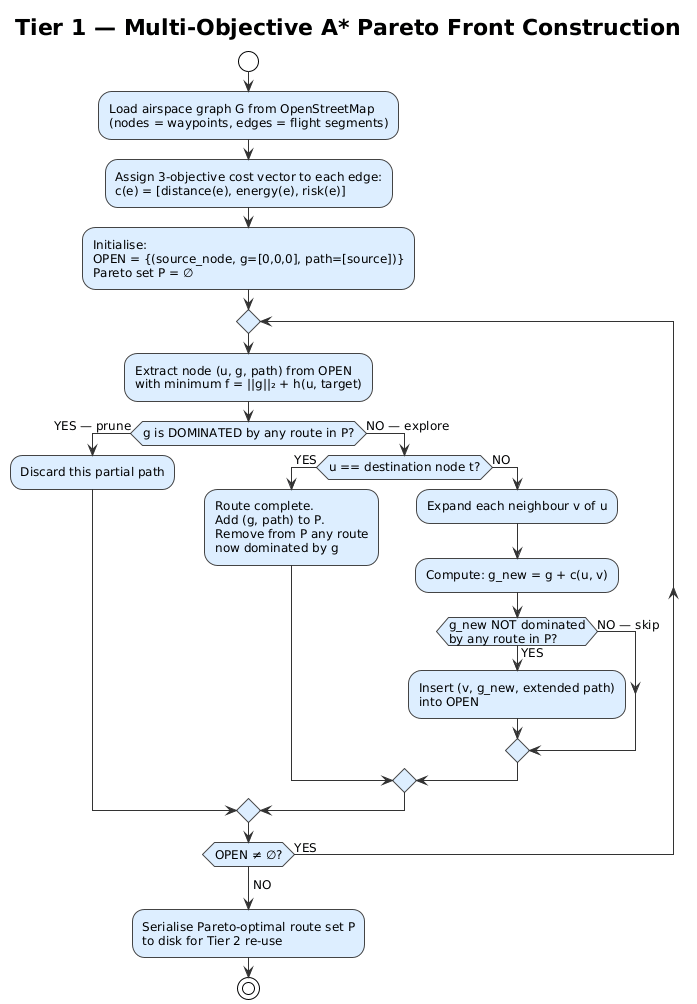
\includegraphics[width=0.70\textwidth]{diagrams/tier1.png}
  \caption{Tier~1 Activity Flow: Multi-Objective A* Pareto Front Construction.
           The open set is explored in order of estimated total cost until no further
           non-dominated routes exist.}
  \label{fig:tier1flow}
\end{figure}

\subsection{Pseudocode: Multi-Objective A* for Pareto Front Construction}

Algorithm~\ref{alg:tier1} presents the pseudocode for Tier~1.

\begin{algorithm}[ht!]
\caption{Multi-Objective A* Pareto Front Construction (Tier~1)}
\label{alg:tier1}
\begin{algorithmic}[1]
\Require Airspace graph $G=(V,E)$ with edge cost vectors
         $\mathbf{c}(e)=[d(e),\epsilon(e),\rho(e)]$,
         source node $s$, destination node $t$
\Ensure  Pareto-optimal route set $\mathcal{P}$

\State $\text{OPEN} \gets \bigl\{\,(s,\;\mathbf{g}=[0,0,0],\;\text{path}=[s])\,\bigr\}$
\State $\mathcal{P} \gets \varnothing$  \Comment{Pareto front (empty initially)}

\While{$\text{OPEN} \neq \varnothing$}
  \State $(u,\,\mathbf{g},\,\text{path}) \gets \text{ExtractMin}(\text{OPEN})$
         \Comment{Min by $f = \|\mathbf{g}\|_2 + h(u,t)$}
  \If{$\mathbf{g}$ is dominated by any route in $\mathcal{P}$}
    \State \textbf{continue} \Comment{Prune dominated paths early}
  \EndIf
  \If{$u = t$}
    \State $\mathcal{P} \gets \text{UpdateParetoFront}(\mathcal{P},\,\mathbf{g},\,\text{path})$
    \Comment{Remove newly dominated routes from $\mathcal{P}$}
  \Else
    \For{each neighbour $v$ of $u$ in $G$}
      \State $\mathbf{g}_{\text{new}} \gets \mathbf{g} + \mathbf{c}(u,v)$
      \If{$\mathbf{g}_{\text{new}}$ is \textbf{not} dominated by any route in $\mathcal{P}$}
        \State $\text{OPEN.insert}\bigl(v,\;\mathbf{g}_{\text{new}},\;\text{path}\cup\{v\}\bigr)$
      \EndIf
    \EndFor
  \EndIf
\EndWhile
\State \Return $\mathcal{P}$ \Comment{Stored to disk for Tier~2 re-use}
\end{algorithmic}
\end{algorithm}

\textbf{Key properties.} The algorithm maintains a cost vector $\mathbf{g}$ (not a
scalar) for each partial path and prunes paths that are dominated by already-discovered
routes. \texttt{UpdateParetoFront} adds the new route and removes any previously stored
routes it dominates. The result is a deterministic, reproducible Pareto front that can be
stored and re-used across all missions in a deployment region.

%% ─────────────────────────────────────────────────────────────────────────────
\section{THE TIER 1--TIER 2 CONNECTION: THE ALGEBRAIC BRIDGE}
\label{sec:bridge}

The connection between Tier~1 and Tier~2 is the central design decision of this project.
This section makes it explicit.

\subsection{Semantic Mapping: From Payload Tags to Routing Objectives}

Each of the four payload metadata tags maps to exactly one Tier~1 routing objective:

\begin{table}[ht!]
\centering
\caption{Semantic Mapping: Payload Metadata Tags to Tier~1 Routing Objectives}
\label{tab:mapping}
\renewcommand{\arraystretch}{1.3}
\begin{tabular}{p{3.0cm}cp{4.0cm}p{5.5cm}}
\toprule
\textbf{Payload Tag} & \textbf{Range} & \textbf{Maps to Tier~1 Objective} & \textbf{Reasoning} \\
\midrule
Fragility class $F$ & $1$--$5$ & $w_{\mathrm{risk}}$ (flight risk weight) &
  Fragile items need low-vibration, low-risk corridors \\
Temperature sensitivity $T$ & $1$--$3$ & $w_{\mathrm{energy}}$ (energy weight) &
  Temp-sensitive items need short exposure time $\rightarrow$ fast flight \\
Delivery urgency $U$ & $1$--$3$ & $w_{\mathrm{dist}}$ (distance weight) &
  Time-critical deliveries need the shortest path \\
Priority level $P$ & $1$--$5$ & Tie-breaker amplifier &
  Scales the dominant weight when scores are close \\
\bottomrule
\end{tabular}
\end{table}

\subsection{Weight Derivation Formula}

From the payload tags, the three routing objective weights are derived
\textbf{algorithmically} with no expert input:

\begin{align}
r_{\text{raw}} &= F \times 2 \label{eq:rraw} \\
d_{\text{raw}} &= U \times 3 \label{eq:draw} \\
e_{\text{raw}} &= T \times 2 \label{eq:eraw}
\end{align}

\begin{align}
w_{\mathrm{risk}}   &= \frac{r_{\text{raw}}}{r_{\text{raw}} + d_{\text{raw}} + e_{\text{raw}}} \label{eq:wrisk} \\
w_{\mathrm{dist}}   &= \frac{d_{\text{raw}}}{r_{\text{raw}} + d_{\text{raw}} + e_{\text{raw}}} \label{eq:wdist} \\
w_{\mathrm{energy}} &= \frac{e_{\text{raw}}}{r_{\text{raw}} + d_{\text{raw}} + e_{\text{raw}}} \label{eq:wenergy}
\end{align}

The multipliers (2 for fragility and temperature, 3 for urgency) reflect the domain
insight that urgency has a higher penalty sensitivity than fragility or thermal
constraints in the UAV medical delivery context.

\subsection{Why This Is Not Extreme-Point Selection}

A critical property of the utility scoring approach (Section~\ref{sec:tier2}) is that it
selects \textbf{different, non-extreme points} for most real payloads. Table~\ref{tab:presets}
demonstrates this for four representative payload presets.

\begin{table}[ht!]
\centering
\caption{Payload Presets and Expected Pareto Point Selection}
\label{tab:presets}
\renewcommand{\arraystretch}{1.3}
\resizebox{\textwidth}{!}{%
\begin{tabular}{lccccccl}
\toprule
\textbf{Payload Preset} & $F$ & $T$ & $U$ &
$w_{\mathrm{risk}}$ & $w_{\mathrm{dist}}$ & $w_{\mathrm{energy}}$ &
\textbf{Expected Selected Point} \\
\midrule
Fragile medical sample  & 5 & 1 & 1 & 0.667 & 0.200 & 0.133 &
  Non-extreme: long, low-risk (NOT the extreme lowest-risk) \\
Emergency medicine      & 1 & 1 & 3 & 0.154 & 0.692 & 0.154 &
  Extreme shortest-distance (correct for this payload) \\
Disaster-relief supplies & 1 & 2 & 1 & 0.222 & 0.333 & 0.444 &
  Non-extreme: energy-optimal intermediate point \\
Mixed cargo             & 3 & 2 & 2 & 0.375 & 0.375 & 0.250 &
  Non-extreme: balanced trade-off \\
\bottomrule
\end{tabular}
}
\end{table}

Only emergency medicine selects an extreme point---and that is the \textit{correct}
answer for that payload. All other mixed-priority payloads select intermediate,
non-extreme points that neither single-objective A* nor MOPSO can produce.

%% ─────────────────────────────────────────────────────────────────────────────
\section{TIER 2 --- PAYLOAD-DRIVEN PARETO SELECTION}
\label{sec:tier2}

\subsection{What Tier 2 Does}

Tier~2 reads the four payload metadata tags assigned by the operator, derives the three
routing objective weights via the formula in Section~\ref{sec:bridge}, normalises the
Pareto front objectives, computes a utility score for every Pareto point, and returns
the $\arg\max$ as the mission route. No weight re-tuning occurs; no planner is re-run.

\subsection{Tier 2 Activity Flow}

Figure~\ref{fig:tier2flow} shows the step-by-step flow of Tier~2.

\begin{figure}[ht!]
  \centering
  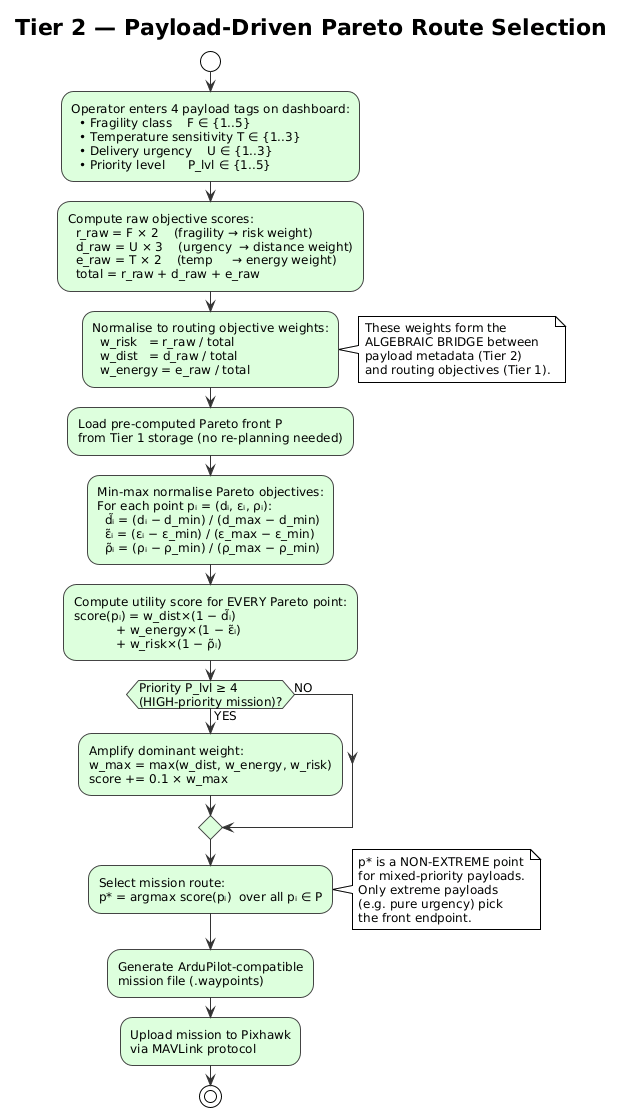
\includegraphics[width=0.65\textwidth]{diagrams/tier2.png}
  \caption{Tier~2 Activity Flow: Payload-Driven Pareto Selection.
           Payload tags are algebraically mapped to weights, which score every Pareto
           point via a utility function; the argmax is selected as the mission route.}
  \label{fig:tier2flow}
\end{figure}

\subsection{Utility Scoring Formula}

For each Pareto point $p_i$ with objective values $(d_i, \epsilon_i, \rho_i)$, the
normalised objective values are:

\begin{equation}
  \tilde{d}_i = \frac{d_i - d_{\min}}{d_{\max} - d_{\min}}, \quad
  \tilde{\epsilon}_i = \frac{\epsilon_i - \epsilon_{\min}}{\epsilon_{\max} - \epsilon_{\min}}, \quad
  \tilde{\rho}_i = \frac{\rho_i - \rho_{\min}}{\rho_{\max} - \rho_{\min}}
\end{equation}

where $d_{\min}, d_{\max}$, etc., are the extremes over the full Pareto front
$\mathcal{P}$. The utility score is:

\begin{equation}
  \text{score}(p_i)
  = w_{\mathrm{dist}} \cdot (1 - \tilde{d}_i)
  + w_{\mathrm{energy}} \cdot (1 - \tilde{\epsilon}_i)
  + w_{\mathrm{risk}} \cdot (1 - \tilde{\rho}_i)
  \label{eq:utility}
\end{equation}

\textbf{Selected route:}
\begin{equation}
  p^* = \arg\max_{p_i \in \mathcal{P}} \;\text{score}(p_i)
\end{equation}

A high $w_{\mathrm{risk}}$ (from a high fragility tag) drives the score to favour points
with low $\tilde{\rho}_i$ (low risk). A high $w_{\mathrm{dist}}$ (from a high urgency
tag) drives the score to favour points with low $\tilde{d}_i$ (short distance). The
formula scores the \textit{entire} Pareto front, not just the extremes.

\subsection{Pseudocode: Payload-Driven Route Selection}

Algorithm~\ref{alg:tier2} presents the complete Tier~2 pseudocode.

\begin{algorithm}[ht!]
\caption{Payload-Driven Pareto Route Selection (Tier~2)}
\label{alg:tier2}
\begin{algorithmic}[1]
\Require Payload tags: Fragility $F \in \{1..5\}$, Temperature $T \in \{1..3\}$,
         Urgency $U \in \{1..3\}$, Priority $P_{\text{lvl}} \in \{1..5\}$
\Require Pre-computed Pareto front $\mathcal{P} = \{(d_i, \epsilon_i, \rho_i)\}_{i=1}^{k}$
\Ensure  Selected mission route $p^*$

\Statex \textbf{--- Step 1: Derive raw scores from payload tags ---}
\State $r_{\text{raw}} \gets F \times 2$
\State $d_{\text{raw}} \gets U \times 3$
\State $e_{\text{raw}} \gets T \times 2$
\State $\text{total} \gets r_{\text{raw}} + d_{\text{raw}} + e_{\text{raw}}$

\Statex \textbf{--- Step 2: Normalise to objective weights ---}
\State $w_{\mathrm{risk}}   \gets r_{\text{raw}} / \text{total}$
\State $w_{\mathrm{dist}}   \gets d_{\text{raw}} / \text{total}$
\State $w_{\mathrm{energy}} \gets e_{\text{raw}} / \text{total}$

\Statex \textbf{--- Step 3: Min-max normalise Pareto objectives ---}
\State $(d_{\min}, d_{\max}) \gets (\min_{p_i \in \mathcal{P}} d_i,\; \max_{p_i \in \mathcal{P}} d_i)$
\State $(\epsilon_{\min}, \epsilon_{\max}) \gets (\min_{p_i} \epsilon_i,\; \max_{p_i} \epsilon_i)$
\State $(\rho_{\min}, \rho_{\max}) \gets (\min_{p_i} \rho_i,\; \max_{p_i} \rho_i)$

\Statex \textbf{--- Step 4: Compute utility score for each Pareto point ---}
\State $\text{best\_score} \gets -\infty$;\quad $p^* \gets \text{null}$
\For{each $p_i = (d_i, \epsilon_i, \rho_i) \in \mathcal{P}$}
  \State $\tilde{d}_i \gets (d_i - d_{\min}) / (d_{\max} - d_{\min})$
  \State $\tilde{\epsilon}_i \gets (\epsilon_i - \epsilon_{\min}) / (\epsilon_{\max} - \epsilon_{\min})$
  \State $\tilde{\rho}_i \gets (\rho_i - \rho_{\min}) / (\rho_{\max} - \rho_{\min})$
  \State $\text{score}_i \gets w_{\mathrm{dist}} \cdot (1 - \tilde{d}_i)
         + w_{\mathrm{energy}} \cdot (1 - \tilde{\epsilon}_i)
         + w_{\mathrm{risk}} \cdot (1 - \tilde{\rho}_i)$
  \If{$P_{\text{lvl}} \geq 4$} \Comment{High-priority: amplify dominant weight}
    \State $w_{\max} \gets \max(w_{\mathrm{dist}}, w_{\mathrm{energy}}, w_{\mathrm{risk}})$
    \State $\text{score}_i \gets \text{score}_i + 0.1 \times w_{\max}$
  \EndIf
  \If{$\text{score}_i > \text{best\_score}$}
    \State $\text{best\_score} \gets \text{score}_i$;\quad $p^* \gets p_i$
  \EndIf
\EndFor
\State \Return $p^*$
\end{algorithmic}
\end{algorithm}

%% ─────────────────────────────────────────────────────────────────────────────
\section{MODULES FOR PHASE I (SOFTWARE SIMULATION)}
\label{sec:phase1modules}

Phase~I delivers a complete, validated software system. The following modules are
implemented, tested, and benchmarked entirely in simulation:

\textbf{Module 1 --- Airspace Graph Builder.} Extracts the road/path network from
OpenStreetMap for a specified delivery region using \texttt{osmnx}. Assigns three
objective costs to each edge: distance (geodesic), energy (distance $\times$
altitude-change factor), and flight risk (simulated threat zones and obstacle density
scored 0--1 using a configurable hazard map).

\textbf{Module 2 --- Multi-Objective A*/Dijkstra Engine (Tier~1).} Implements
Algorithm~\ref{alg:tier1} using Python and NetworkX \cite{networkx}. Produces a
Pareto-optimal route set stored as a serialised Python object. The module includes unit
tests that verify Pareto non-dominance of all returned routes.

\textbf{Module 3 --- MOPSO Baseline.} Implements a Multi-Objective Particle Swarm
Optimisation baseline \cite{mopso} with swarm size 100, 200 iterations, and a Pareto
archive of 100 solutions. Used to benchmark Tier~1 on hypervolume and Pareto spread.

\textbf{Module 4 --- Payload Metadata Interpreter (Tier~2).} Implements
Algorithm~\ref{alg:tier2}: reads the four payload tags, derives objective weights via
Equations~(\ref{eq:wrisk})--(\ref{eq:wenergy}), applies utility scoring
(Equation~(\ref{eq:utility})), and returns the $\arg\max$ route.

\textbf{Module 5 --- Benchmarking Suite.} Evaluates all methods on three scenario scales:
S1 ($\sim$50 nodes, low obstacle density), S2 ($\sim$200 nodes, medium density),
and S3 ($\sim$500 nodes, high density). Metrics: Hypervolume (HV), Inverted
Generational Distance (IGD), and Tier~2 selection accuracy across four payload presets.
MOPSO runs 30 times per scenario to obtain mean $\pm$ standard deviation.

\textbf{Module 6 --- Ground-Station Dashboard.} A Tkinter or React operator interface
where the operator enters the four payload tags once. The system automatically selects
the route from the pre-computed Pareto front and generates an ArduPilot-compatible
mission file (\texttt{.waypoints}) for upload to the UAV.

%% ─────────────────────────────────────────────────────────────────────────────
\section{MODULES FOR PHASE II (HARDWARE IMPLEMENTATION)}
\label{sec:phase2modules}

Phase~II deploys the validated software system onto physical hardware and conducts
outdoor flight tests:

\textbf{Module 7 --- Raspberry Pi 5 Integration.} Ports the Tier~1 and Tier~2 Python
modules to the onboard Raspberry Pi~5. Verifies that Tier~1 pre-computation runs within
acceptable time on the onboard CPU, and that Tier~2 route selection is near-instantaneous
($<$1\,s end-to-end from payload tag input to mission file output).

\textbf{Module 8 --- MAVLink Mission Upload.} Implements MAVLink \cite{mavlink}
communication between the Raspberry Pi and the Pixhawk flight controller. Converts the
selected Pareto route into ArduPilot-compatible waypoint format and uploads it to the
Pixhawk via the MAVLink protocol in real time.

\textbf{Module 9 --- ArduPilot SITL Validation (Pre-flight).} Before any real flight,
all routes selected by Tier~2 are validated in ArduPilot's Software-in-the-Loop (SITL)
simulation. SITL faithfully emulates the Pixhawk's flight controller software, allowing
end-to-end validation of the route adherence behaviour without hardware risk.

\textbf{Module 10 --- Outdoor Flight Tests.} Real outdoor flights on the F450 quadcopter
frame with Pixhawk flight controller. Measures route adherence (GPS position error
vs.\ planned route), end-to-end latency (payload tag entry to mission upload), and
payload delivery success rate across all three payload presets (fragile, emergency,
disaster-relief).

%% ─────────────────────────────────────────────────────────────────────────────
\section{TOOLS AND TECHNOLOGY STACK}

Table~\ref{tab:tools} summarises the full tools and software stack.

\begin{table}[ht!]
\centering
\caption{Tools and Technology Stack}
\label{tab:tools}
\renewcommand{\arraystretch}{1.3}
\begin{tabular}{ll}
\toprule
\textbf{Component} & \textbf{Tool / Library} \\
\midrule
Graph construction      & osmnx (Python), OpenStreetMap data \\
Multi-objective search  & Python, NetworkX \cite{networkx} \\
Objective computation   & NumPy \\
Pareto front storage    & Python serialisation (pickle / JSON) \\
Visualisation           & Matplotlib, custom interactive HTML \\
MOPSO baseline          & Python (custom implementation) \cite{mopso} \\
UAV mission upload      & ArduPilot Mission Planner, MAVLink \cite{mavlink, ardupilot} \\
Ground-station UI       & Tkinter (Phase~I); React (optional Phase~II) \\
Onboard compute         & Raspberry Pi~5 \\
Flight controller       & Pixhawk (ArduPilot firmware) \\
UAV frame               & F450 quadcopter \\
\bottomrule
\end{tabular}
\end{table}